\label{sec:2_problem_and_application}
\section{Problem and application}
% Problem:
\subsection{Problem}
% ------------------------------------------

% Black-box
Even though these deep networks have made big positive achievements in domains like object detection \cite{girshickRichFeatureHierarchies2014, renFasterRCNNRealTime2015, redmonYouOnlyLook2016, linFocalLossDense2017}, image annotation, and captioning \cite{vinyalsShowTellNeural2015, karpathyDeepVisualSemanticAlignments2015, johnsonDenseCapFullyConvolutional2016, tranRichImageCaptioning2016}, it is with their complexity harder to understand why these networks predict what they do. Humans, both researchers and users, of these systems need to be able to understand how these black-box algorithms work in order to gain trust \cite{koehlerExplanationImaginationConfidence1991, herlockerExplainingCollaborativeFiltering2000, dzindoletRoleTrustAutomation2003}, improve the models and apply these networks in new ways and domains \cite{jiangArtificialIntelligenceHealthcare2017, tonekaboniWhatCliniciansWant2019, holzingerCausabilityExplainabilityArtificial2019, guptaDeepLearningObject2021, tjoaSurveyExplainableArtificial2021}. Researchers and model architects can understand how the information flows in the network on a higher level. However, when the architecture gets larger, deeper, and more complex, and the training datasets are getting larger, it can be challenging to understand what input data contributed to making the decision \cite{sagirogluBigDataReview2013}.

% Interpretablity vs accuracy 
The models with the highest accuracies on large datasets, often have so complex architectures, that even domain experts struggle to interpret their decision \cite{caruanaIntelligibleModelsHealthCare2015}. Meanwhile, smaller, less complex architectures often have less accuracy and generalize poorer than their more complex counterparts. An example of this was shown in a case study to predict how severe the risk of dying was for patients with pneumonia, to assist healthcare workers to prioritize \cite{cooperPredictingDireOutcomes2005}. They found the most accurate model to be a neural net, which outperformed less complex models, such as logistic regression. A rule-based system was also evaluated, and although this is a simpler model than neural nets, it is interpretable by design. This rule-based model showed that if a patient had both pneumonia and asthma, it had a lower chance of dying in relation to just having pneumonia, and therefore less important to treat. The reason for this conclusion was that patients in the training dataset who had both pneumonia and asthma were usually prioritized first, and therefore had a higher survival rate \cite{cooperEvaluationMachinelearningMethods1997}. Because of this insight from the rule-based method, more complex models, such as neural nets, were concluded to be too risky.

In the pursuit of models with higher accuracies, the main way to achieve this is with even more complex models and larger training datasets \cite{bianchiniComplexityNeuralNetwork2014}. This brings the trade-off of an interpretable and explainable model vs. a more accurate model \cite{barredoarrietaExplainableArtificialIntelligence2020} to the forefront of discussion. 


% XAI
The field of \gls{xai} is working on solving the trade-off between performance and explainability. Some approaches specialize in explaining specific architectures, called model-specific. Meanwhile, others, called model-agnostic, try to explain models of different architectures, exploiting inherent properties in neural networks and statistics. Examples of models that are inherently explainable, like decision trees, Bayesian classifiers, logistic regression, linear models, and \gls{knn} \cite{fixDiscriminatoryAnalysisNonparametric1989, coverNearestNeighborPattern1967}, are interpretable, and hereby explainable, by design. This is because their internal structure and computations follow clear rules or formulas that are manageable to comprehend.
Models such as deep neural networks can however work better than less complex methods on larger datasets. Because of their complex structure, with many hidden layers and weights trained on large datasets, it is difficult, if not impossible for humans to understand what the model evaluated when choosing a prediction. To better understand these complex methods, researchers in \gls{xai} have developed methods that are both model-specific and post-hoc model-agnostic techniques that can explain the underlying model prediction. These methods try to bridge the gap between high accuracies and explainability.
In theory, this allows us to use the model best fit for the task, regardless of complexity, and without the expense of not understanding the model's predictions. 

% Many models 
Different explanations try to give different insights into the predictions. Local explanation looks at one specific decision of the model and tries to explain what was important in the input data to give this prediction. Global explanation on the other hand looks at the whole model's process of making decisions and sees how the different attributes contribute to making a decision. These global explanations can also be built from multiple local faithful explanations. A third type is contrastive explanations that utilize local features to explain the difference between instances. This allows insight into the inner workings of the model on a more global scale, based on local predictions.

% Cons
One typical disadvantage of model-agnostic explanations is that the insights and explanations they give, are not always faithful to the underlying model they try to explain. This can happen if an explaining model is trained to look at the underlying model's input, inner workings, and output, and learns the correlation between them. The problem then is that correlation does not imply causation and the explaining model can give a deceiving explanation, that can look correct at first. \gls{xai} researchers work hard and try to find more underlying features of statistics so that the explaining model does learn the causation, and not only the correlation.




% Application (where my system will go):
\subsection{Application}
% ------------------------------------------

% Intro
With better explanations, that are both intuitive and faithful to the underlying prediction model, humans can be more precise when making improvements to the model. This also gives the ability to use the model with confidence that the prediction is based on correct decisions.


% Medical / bank
When machine learning methods are utilized as a tool in the real world, it is important that everyone in the process of using the tool can trust the model. 
In a medical setting, both the doctor and the patient need to have trust that the conclusion taken is based on a reasonable and trustworthy basis. If the model is correct, but the doctor does not have trust in the underlying model, or the patient does not have an explanation of the conclusion taken by the model, the model will not be used as intended, and therefore is a useless tool. 

This is also the case in other domains, such as a bank. Here the bank can utilize large models that look at the person applying for a loan using big data. The bank can make a profile on the customer, alongside fellow citizens in the same demographic, and use a model to predict if this customer should get a loan or not. In this case, it can be difficult to find all biases in the dataset, since it can be hard to distinguish correlation from causation in demographic analysis. Here it is necessary for the bank to have an explanation alongside the predicted output of the loan, to better see if the model made a trustworthy decision. 

% Non-experts improve models



% Finding bias in datasets
One great advantage of being able to better understand the model's evaluations in a prediction is that it can show biases in the dataset. If these biases are known and understood, they can be combated. Ribeiro et al. \cite{ribeiroWhyShouldTrust2016} showed that it can be hard to discover biases when the predictions are correct, without knowing the reasoning. They carried out an experiment with a model trained on images of huskies and wolfs and first presented the model's prediction without explanations to participants. The participants were then asked to determine if they trusted the model or not. Thereafter the model's explanation for the predictions was presented and participants again had to tell if they trusted the model now. In both instances, the participants were also asked if they thought snow was a potential feature of importance. An image of a husky misclassified as a wolf can be seen in Figure \ref{fig:wolf_husky}, alongside the regions important in making the decision. The results can be seen in Table \ref{table:husky_vs_wolf}, and it can be seen that a considerable amount of the participants lost trust in the biased model when they were presented with the explanation. They then saw that the decision was based only on whether the snow was visible in the image or not. This shows that models with an intuitive explanation are more likely to gain the trust of their users. Trustworthy explanations open the ability for users who do not have insight into the making of the model, to still be able to detect biases in the dataset and improve the model. 

\begin{table}[htb]
    \centering
    \begin{tabular}{ c c c} 
     
               & Before explanation & After explanation\\ [0.5ex] 
        \Xhline{1.5pt} \\ 
            Trusted the biased model & 10 out of 27 & 3 out of 27 \\  [0.5ex]
        \hline  \\ 
            Thought snow was an \\ important feature & 12 out of 27 & 25 out of 27 \\ [1ex] 
        \hline
    \end{tabular}
    \caption[Overview over the trust by participants in the "Husky vs. Wolf" experiment by Ribeiro et al. \cite{ribeiroWhyShouldTrust2016}.]{Overview over the trust by participants in the "Husky vs. Wolf" experiment by Ribeiro et al. \cite{ribeiroWhyShouldTrust2016}. The majority lost trust when explained that a classifier considered snow in the background as the most important feature when classifying images of huskies and wolves.}
    \label{table:husky_vs_wolf}
\end{table}

\begin{figure}[htb]
    \centering
    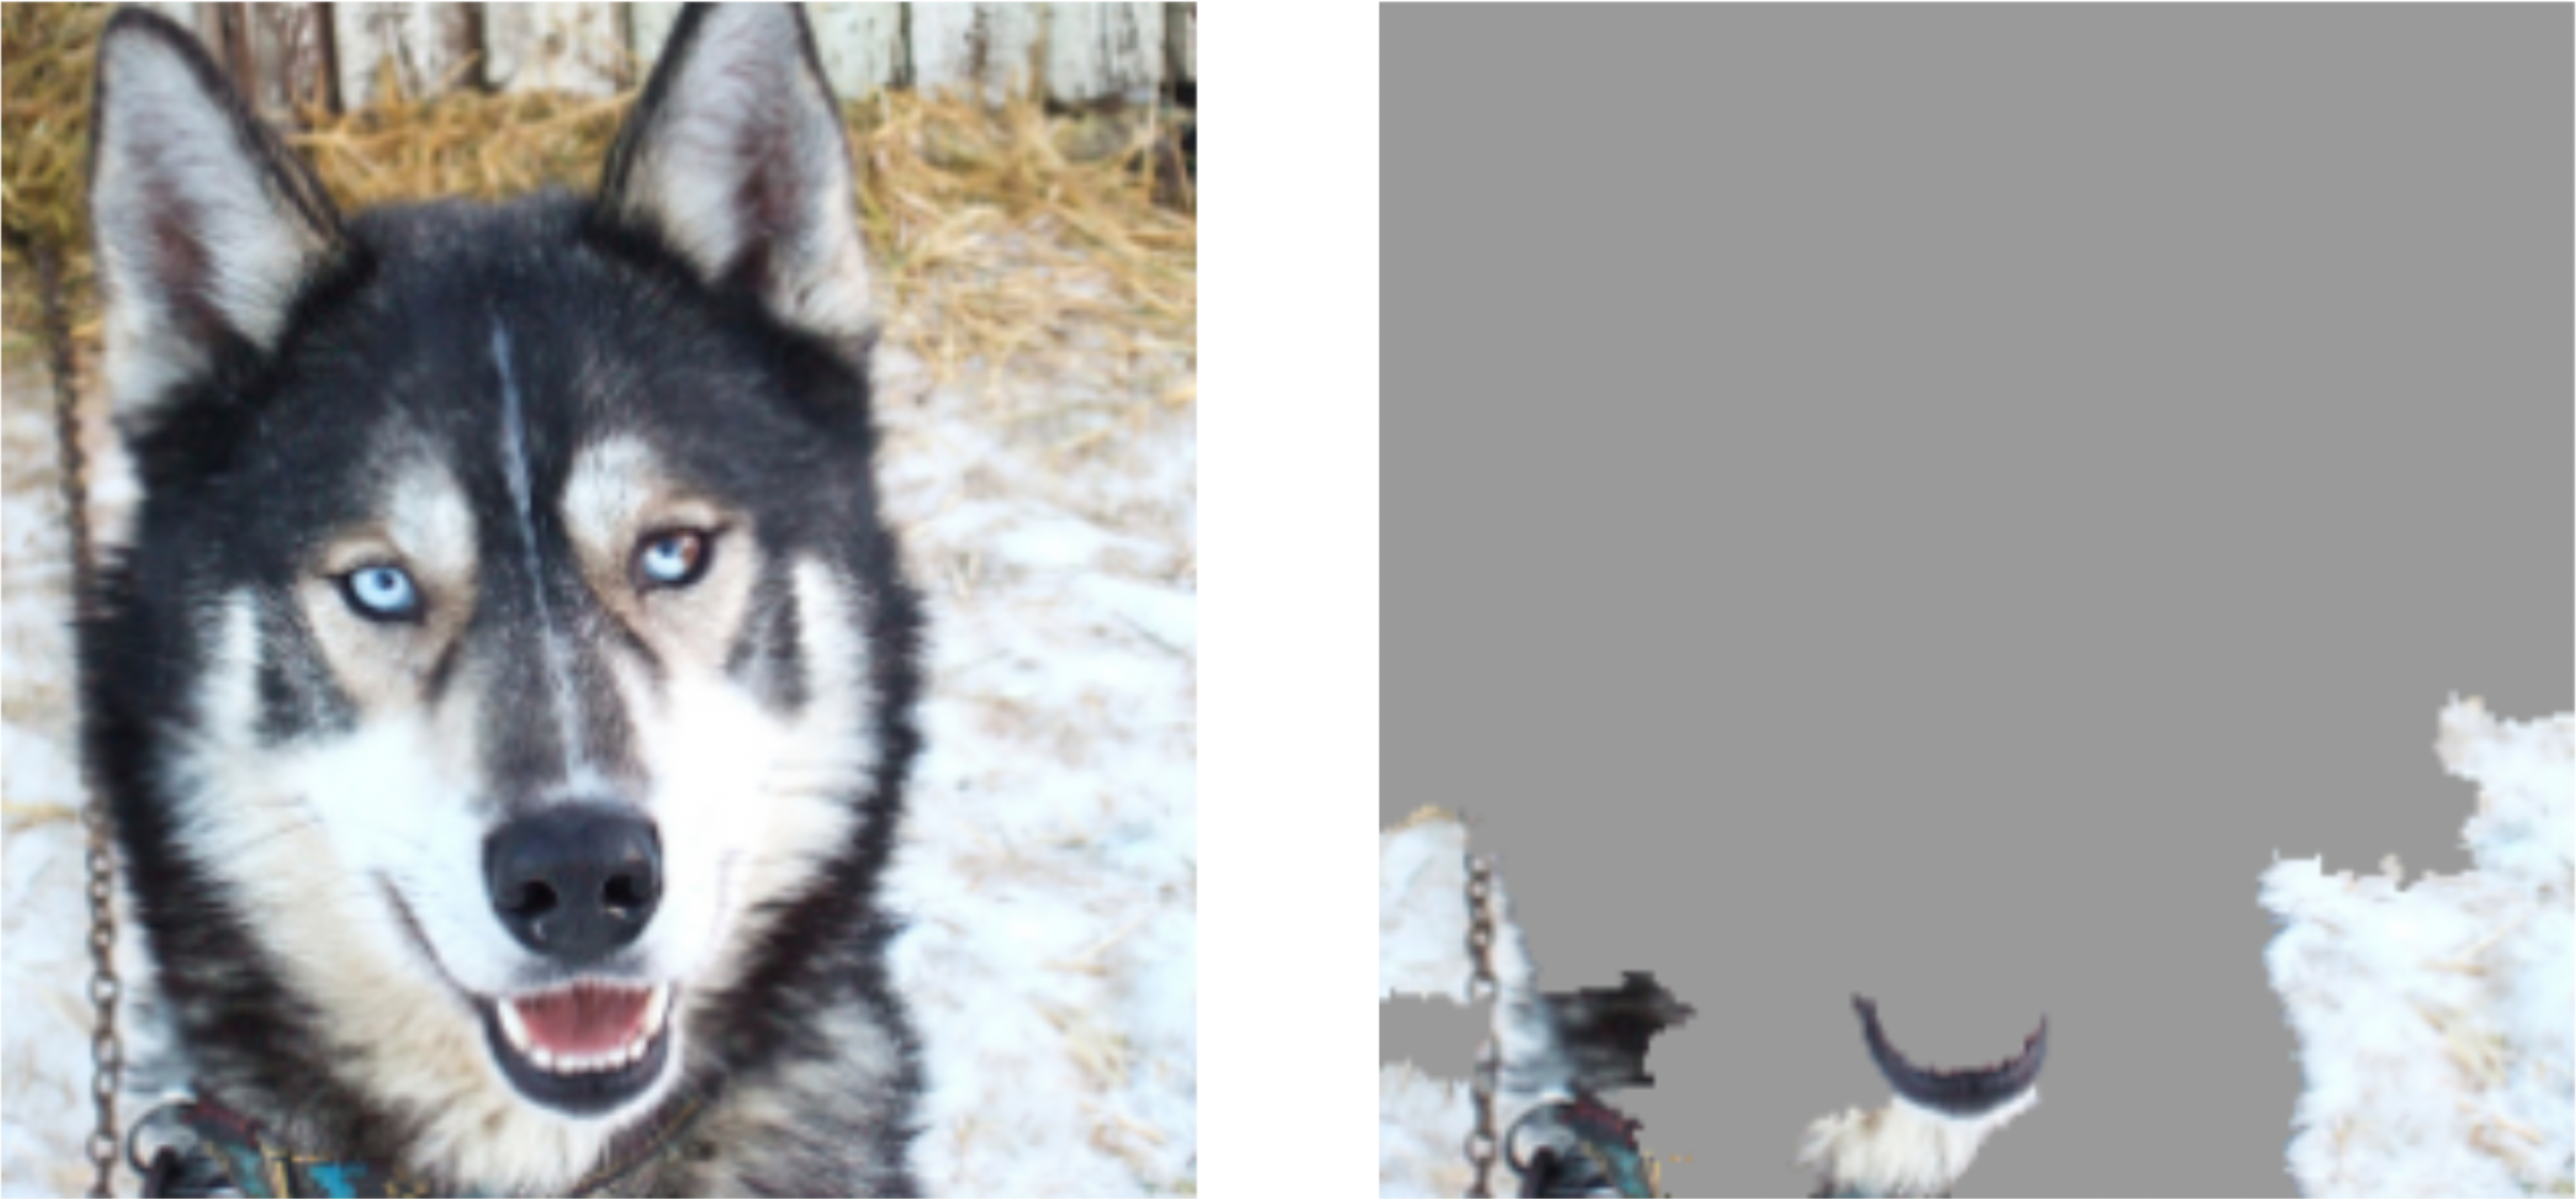
\includegraphics[width=\linewidth]{images/husky_vs_wolf.png}
    \caption[Husky classified as a wolf, alongside an explanation of what the model considered important.]{Husky classified as a wolf, alongside an explanation of what the model considered important. Image by Ribeiro et al. \cite{ribeiroWhyShouldTrust2016}.}
    \label{fig:wolf_husky}
\end{figure} 


% Make humans able to learn from the models
Some machine learning models today are already better than humans in domain-specific tasks, like chess \cite{campbellDeepBlue2002}. Silver et al. \cite{silverGeneralReinforcementLearning2018} proposed the reinforcement learning algorithm AlphaZero, which learns to play chess, shogi (Japanese chess), and Go, only by playing with itself. This method does not get any domain knowledge except the game rules and achieves performance better than humans. Because this algorithm has not seen humans play these games, it does not have human biases and playing flaws in it, and professional game players can learn new moves and techniques by playing with it. 
As superhuman performance is a goal to strive for when it comes to machine learning, it is more important than ever that these algorithms give explanations on what they do and why so that humans can learn new aspects never before thought of.
